\documentclass[article]{jss}\usepackage[]{graphicx}\usepackage[]{color}
%% maxwidth is the original width if it is less than linewidth
%% otherwise use linewidth (to make sure the graphics do not exceed the margin)
\makeatletter
\def\maxwidth{ %
  \ifdim\Gin@nat@width>\linewidth
    \linewidth
  \else
    \Gin@nat@width
  \fi
}
\makeatother

\usepackage{Sweave}


\usepackage[sumlimits, intlimits, namelimits]{amsmath}
\usepackage{soul}

%% later to include the paper as vignette use:
%% \documentclass[nojss]{jss}

\newcommand{\tj}[1]{\textcolor{red}{#1}}


\usepackage[colorinlistoftodos,prependcaption,textsize=tiny]{todonotes}
\presetkeys%
    {todonotes}%
    {inline,backgroundcolor=yellow}{}
    
\makeatletter
\if@todonotes@disabled
\newcommand{\hlfix}[2]{#1}
\else
\newcommand{\hlfix}[2]{\texthl{#1}\todo{#2}}
\fi
\makeatother

%%%%%%%%%%%%%%%%%%%%%%%%%%%%%%
%% declarations for jss.cls %%%%%%%%%%%%%%%%%%%%%%%%%%%%%%%%%%%%%%%%%%
%%%%%%%%%%%%%%%%%%%%%%%%%%%%%%

%% to get the default layout:



%% almost as usual
\author{Daniel Saban\'es Bov\'e\\Hoffmann-La Roche Ltd \And
        Wai Yin Yeung\\Hoffmann-La Roche Ltd \And
        Giuseppe Palermo\\Hoffmann-La Roche Ltd \And
        Thomas Jaki\\Lancaster University}
\title{Model-based Dose Escalation Designs in \proglang{R} with \pkg{crmPack}}

%% for pretty printing and a nice hypersummary also set:
\Plainauthor{Daniel Saban\'es Bov\'e,
    Wai Yin Yeung,
    Giuseppe Palermo,
    Thomas Jaki} %% comma-separated
\Plaintitle{Model-based Dose Escalation Designs in R with crmPack} %% without formatting
\Shorttitle{\pkg{crmPack}: Model-based Dose Escalation} %% a short title (if necessary)

%% an abstract and keywords
\Abstract{
  Model-based dose escalation designs have gained increasing interest due to the
  need for more efficient and informative Phase I trials. The wide-spread
  implementation of such designs has been hindered by the need for either
  licensing specialized commercial software or programming the design and
  simulations from scratch for each project. The \proglang{R}-package \pkg{crmPack} 
  provides a simple and unified object-oriented framework for model-based dose escalation
  designs. This enables the standard use of such designs, while being able to 
  flexibly adapt and extend them. The framework comprises classes and methods 
  for the data structure including the dose grid, statistical models including  
  prior specification, rules for maximum increments, next best dose, and adaptive
  stopping and cohort sizes. In addition to multiple modified classic
  continual reassessment method and escalation with overdose control
  designs with possibly advanced prior specifications 
  (e.g., minimal informative and mixture priors), \pkg{crmPack} currently features dual-endpoint 
  (safety and biomarker) designs and two-part designs. 
  Optional assignment of a small number of patients in each cohort to 
  placebo instead of treatment enables the use in trials outside Oncology. 
%   We introduce \pkg{crmPack} by outlining the design framework and show how easy it is
% to specify a design, run simulations, and report dose recommendations during the
% trial.
}
\Keywords{continual reassessment method, model based dose escalation, dual-endpoint design, \proglang{R}, object oriented}
\Plainkeywords{continual reassessment method, model based dose escalation, dual-endpoint design, R, object oriented} %% without formatting
%% at least one keyword must be supplied

%% publication information
%% NOTE: Typically, this can be left commented and will be filled out by the technical editor
%% \Volume{50}
%% \Issue{9}
%% \Month{June}
%% \Year{2012}
%% \Submitdate{2012-06-04}
%% \Acceptdate{2012-06-04}

%% The address of (at least) one author should be given
%% in the following format:
\Address{
  Daniel Saban\'es Bov\'e\\
  F. Hoffmann-La Roche Ltd\\
  Product Development Biostatistics\\
  Grenzacherstrasse 124\\
  4070 Basel, Switzerland\\
  E-mail: \email{sabanesd@roche.com}\\
  Telephone: +41/61/68-73470
}
%% It is also possible to add a telephone and fax number
%% before the e-mail in the following format:
%% Telephone: +43/512/507-7103
%% Fax: +43/512/507-2851

%% for those who use Sweave please include the following line (with % symbols):
\usepackage{Sweave}

%% end of declarations %%%%%%%%%%%%%%%%%%%%%%%%%%%%%%%%%%%%%%%%%%%%%%%

% custom commands:
\newcommand{\given}{\,\vert\,}
\IfFileExists{upquote.sty}{\usepackage{upquote}}{}
\begin{document}

%% include your article here, just as usual
%% Note that you should use the \pkg{}, \proglang{} and \code{} commands.

%%\section[About Java]{About \proglang{Java}}
%% Note: If there is markup in \(sub)section, then it has to be escape as above.

\section{Introduction}
\label{sec:introduction}

Phase I trials that are testing new investigational agents in humans 
for the first time escalate from low to high doses in a sequential fashion. 
This dose escalation design is necessary
in order to reduce the risk of too high and therefore too toxic doses for the probands. 
These can either be healthy volunteers (e.g., in neurology) or patients
(e.g., in oncology), and we will henceforth use only the latter for ease of
presentation. While higher doses of agents are usually expected to deliver
stronger pharmacodynamic effects and hence improved efficacy, higher doses also
usually cause more severe adverse events in the patients. In order to simplify
the decision making usually binary dose-limiting toxicities (DLTs) are defined
(e.g., adverse events reaching specific severity levels) before starting the
trial. The maximum tolerated dose (MTD) is then defined as the dose with a
certain probability of DLTs (either using a single value, e.g., 33\%, or a
range, e.g., 20 to 35\%). Historically, patients were treated at the same
dose in cohorts of three, with the dose for the next cohort then being
determined from the number of DLTs having been observed in the current cohort.

Algorithmic designs like the simple 3+3 design \citep{carter1973} have
disadvantages that have been recognized in the statistics community, see e.g.,
\cite{Paoletti2015}. Fundamentally, the escalation rules of the 3+3 design do
not have any statistical justification \citep{Storer1989} in terms of estimating
an MTD. Moreover, they cannot be extended to address today's Phase I trials,
with extension cohorts, dose escalation of drug combinations and optimal
biological dose determination, naming just a few prominent challenges. Hence
model-based dose escalation designs like the continual reassessment method
\citep[CRM,][]{oquigley1990} have gained increasing interest due to the need for
more efficient and informative Phase I trials. These designs are based in
statistical inference, with dose-toxicity regression models as the backbone, and
are therefore flexible for adaptation to various complex trial designs.
Importantly, they avoid fixing only a few dose levels in advance. For a wider comparison of algorithmic and model based designs see e.g., \cite{jaki2013}.

However, the wide-spread implementation of such designs has been hindered by the
need for either licensing specialized commercial software (thus losing
flexibility) or programming the design and simulations from scratch for each
project (thus losing efficiency). While the models underlying most model-based
dose escalation procedures can easily be fit in standard software with the
capability to fit generalized linear models, e.g., \pkg{PROC MIXED} in
\proglang{SAS} \citep{SAS2003}, \pkg{glm} in \proglang{Stata} \citep{Stata2015} or \proglang{R} \citep{R2016}, 
there are still only few software solutions available dedicated to dose escalation studies.

The commercial packages \proglang{East} \citep{East2016} and
\proglang{ADDPLAN} \citep{Addplan2016} both offer extensions to their basic
design software for dose escalation studies (\pkg{ESCALATE} in \proglang{East}
and \pkg{df} in \proglang{ADDPLAN}) implementing the algorithmic 3+3 design and
various versions of the CRM. Similarly \proglang{FACTS} \citep{FACTS} also
offers different common dose escalation methods. Due to the commercial nature of
these implementations there is, however, a limitation on how much the designs
can be tailored towards the individual needs of the study. Similarly static
implementations of methods for dose escalation are available in the
\proglang{Stata} module \pkg{crm} \citep{StataCRM} which implements the CRM and
the  \pkg{dfcrm} package \citep{dfcrm2013} in \proglang{R} which additionally implements the
time-to-event CRM (TITE-CRM) \citep{cheung2000}. Several \proglang{R}-packages 
with extensions are available. The \pkg{bcrm} package \citep{sweeting2013} implements a variety of one and two parameter models, and facilitates different
ways to specify prior distributions, escalation and stopping rules. The \pkg{ordcrm} package
\citep{ordcrm} implements ordinal proportional odds and continuation ratio models for CRMs. 
The \pkg{dfpk} package \citep{dfpk} uses pharmacokinetic data in the dose escalation.

In this paper we introduce the \proglang{R}-package \pkg{crmPack} \citep{crmPack} for
dose escalation studies, which is publicly available on CRAN. While the package's name
pays tribute to the original CRM as the first model-based dose escalation design, the 
package's functionality differs from the above existing implementations in
three fundamental ways. Firstly, it is written using \proglang{S4} classes and methods
\citep{Chambers2008}, which allows customized methodology to be added to the
package while still being able to use the existing backbone functionalities.
Secondly, methods for studies with a placebo group (e.g., for healthy volunteer
studies) are readily implemented. Thirdly, dual endpoint dose escalation methods
that incorporate both safety and efficacy and allow determination of an optimal
biological dose are already available. 

\section{Framework}\label{sec:framework}

For describing the framework of the package we will adapt the general notation
for early phase trials from \cite{Thall2010}. Figure~\ref{fig:schematic} summarizes
the framework in a schematic.

\begin{figure}
\centering 
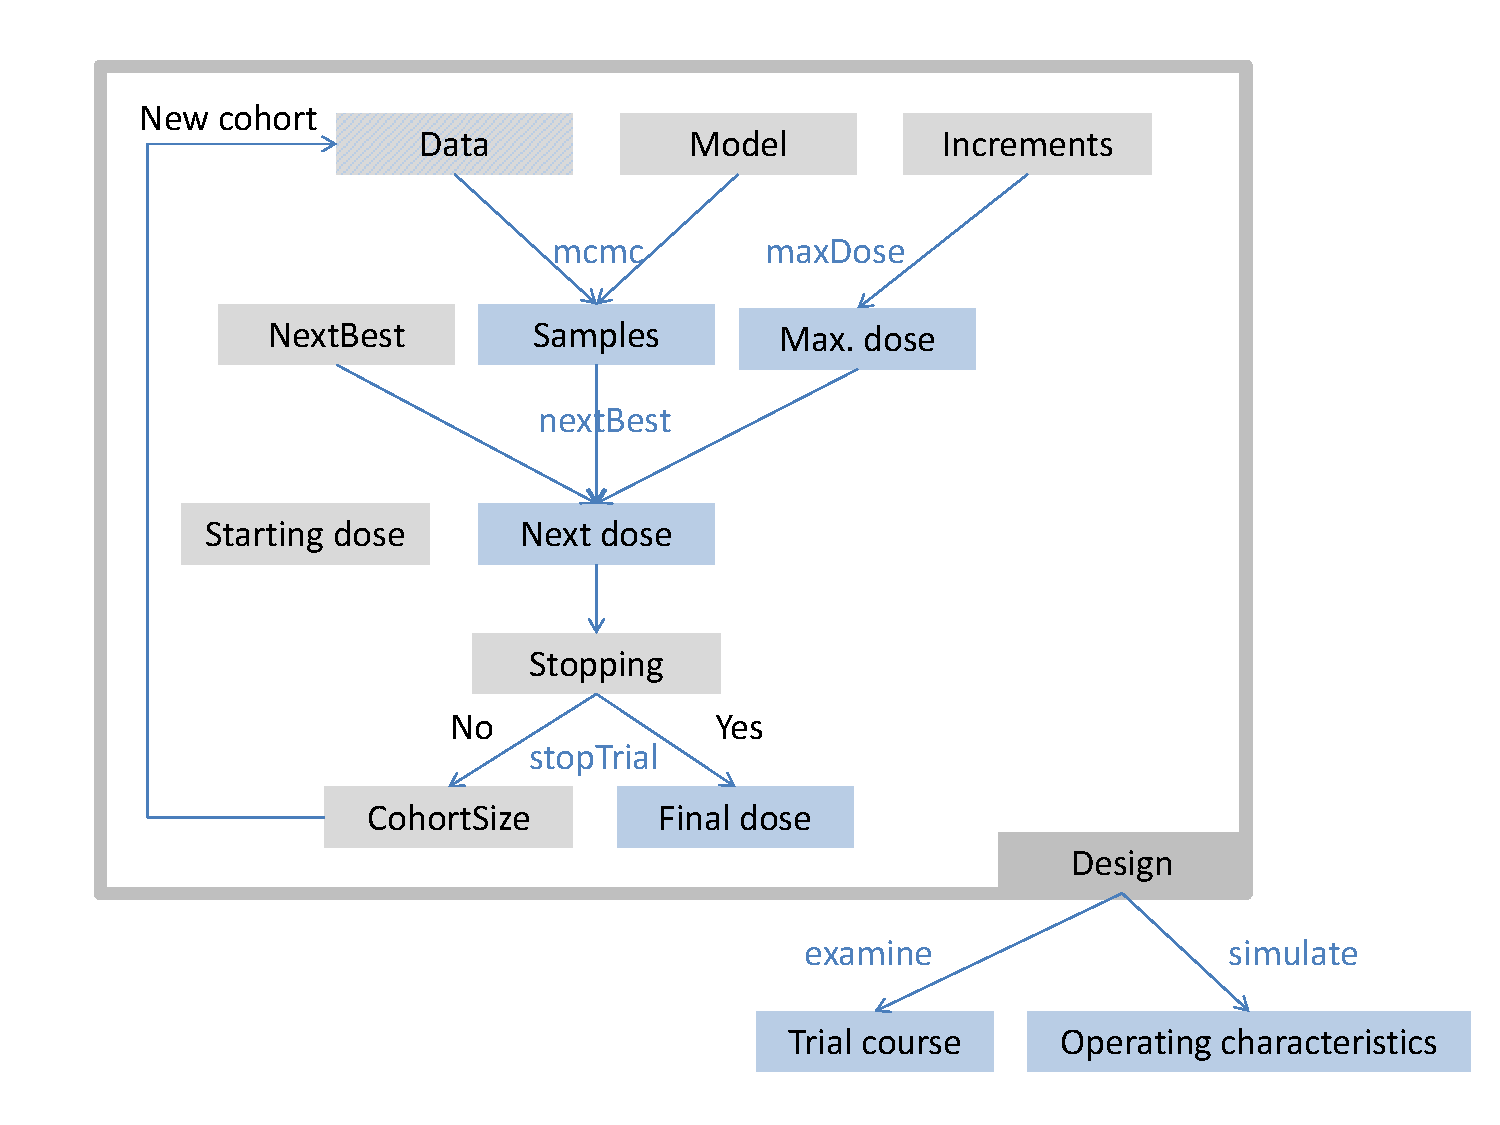
\includegraphics[width=.8\linewidth]{schematic.pdf} 
\caption{Schematic of the framework. Separate design features are implemented as classes
(shown as gray boxes) and bundled together in the overarching \code{Design} object. 
They can be processed with various methods (blue text) to run the dose escalation trial and produce results (blue boxes). For example, the \code{Data} and \code{Model} objects can be processed by the \code{mcmc} method in order to obtain posterior samples of the model parameters, and given the sample size and the dose for the next cohort, the updated \code{Data} closes the dose escalation loop. On the higher level, designs can be investigated with the \code{examine} and \code{simulate} methods to obtain hypothetical trial courses and operating characteristics, respectively. Note that individual model classes and methods are not shown here for clarity, please refer to the package documentation for details, e.g., by calling \code{crmPackHelp()}.} 
\label{fig:schematic}
\end{figure}

\paragraph{Data}
\label{sec:frame:data}
%
Let $x$ denote one specific treatment, chosen from the set
of possible treatments ${\cal X}$. This could be one specific dose, but also
more generally a vector, containing for example doses of multiple drugs in a
combination trial. After giving treatment $x$ to a patient, the outcome $y$
is observed, typically a safety endpoint as e.g., the binary DLT $y \in \{0,
1\}$. Grouping together $n_{j}$ patients in cohort $j$, generating the cohort
$j$ data ${\cal C}_{j} = \{(x_{j}, y_{j,1}), \dotsc, (x_{j},
y_{j,n_{j}})\}$, we can denote the data generated from the first $N$ cohorts as
${\cal D}_{N}= {\cal C}_{1} \cup \dotsb \cup {\cal C}_{N}$.
%
In \pkg{crmPack} the \proglang{S4} class \code{GeneralData} encapsulates this
notion and subclasses implement concrete data structures.

\paragraph{Model}
\label{sec:frame:model}
%
The core of model-based dose escalation designs is the underlying statistical model. Taking a
Bayesian approach to inference, the model in \pkg{crmPack} consists of firstly the
likelihood, which is either a probability density function $f(y \given x,
\theta)$ or a probability mass function $\Prob(Y=y \given x, \theta)$ of $y$ for
a patient who receives treatment $x$ assuming the parameter (vector) $\theta$,
% (this is the likelihood of $\theta$)
and secondly the prior $p(\theta \given \xi)$ for $\theta$ given fixed
hyperparameters $\xi$.
%
In \pkg{crmPack} the virtual \proglang{S4} class \code{AllModels} encapsulates this
notion and subclasses implement concrete models.

For example, the class \code{LogisticLogNormal} implements
the logistic regression model \citep{Neuenschwander2008} with
\begin{equation}
\label{eq:LogisticLogNormal}
\mathrm{logit}(\Prob(Y=1 \given x,\theta))
\equiv \mathrm{logit}(\pi(x,\theta))
= \alpha_{0} + \alpha_{1} \log\left(\frac{x}{x^*}\right),
\end{equation}
parameter vector $\theta = (\alpha_{0},\alpha_{1})$, dose $x > 0$ and specified
reference dose $x^{*}$. The prior $p(\theta \given \xi)$ is specified
via a bivariate normal distribution on a transformation of $\theta$ to ensure
$\alpha_{1} > 0$:
\begin{equation}
  \label{eq:bivariateNormal}
  (\alpha_{0}, \log(\alpha_{1})) \given \xi \sim \mathcal{N}_{2} (\mu, \Sigma)
\end{equation}
with hyperparameters $\xi = (\mu, \Sigma)$ consisting of the prior mean vector
$\mu$ and the prior covariance matrix $\Sigma$.

\paragraph{Decision making for the next dose}
\label{sec:frame:decision-making}
%
Another core element of a dose escalation design concerns the decision making
for the next dose $x_{N+1}$ to be tested in the next cohort $N+1$. In the
\cite{Thall2010} notation, the function $\alpha$ is mapping the currently
accumulated data $\mathcal{D}_{N}$ to the dose space $\mathcal{X}$ (or to dose
$0$, meaning to stop the trial because all doses are too toxic):
\begin{equation}
\alpha: {\cal D}_{N} \rightarrow \mathcal{X} \cup \{0\}
\end{equation}
This mapping is commonly specified via the combination of two elements:
The first element is a function $\tau$ for the maximum increments between dose
levels, which can calculate from the current data $\mathcal{D}_{N}$ (including the
current dose $x_{N}$) the maximum possible next dose $t_{N+1}=\tau(\mathcal{D}_{N})$ 
for the next cohort. The second element is a rule $\nu$ indirectly
acting on the current data through the posterior distribution $p(\theta \given
\mathcal{D}_{N})$ and the maximum possible dose $t_{N+1}$ to finally give the
next dose $x_{N+1} = \nu(p(\theta \given \mathcal{D}_{N}), t_{N+1})$.
%
In \pkg{crmPack} maximum increments are specified by subclasses of
\code{Increments}, and the next best dose rule by subclasses of \code{NextBest}.

\paragraph{The design class}
\label{sec:frame:design}
%
Additional features of a design concern the adaptive sizing of the next
cohort and the adaptive stopping of the trial. Those are implemented in
subclasses of \code{CohortSize} and \code{Stopping}, respectively.
Moreover, the starting dose $x_{1}$ is also a feature of the design.
%
Finally, the overall dose escalation design is bundling all the described
features together in a dedicated class typically inheriting from \code{Design}.
%
As noted in \cite{Thall2010}, the operating characteristics of such a complex
dose escalation design can only be evaluated by simulations. This can be done
using the \code{simulate} methods for the design classes, and is recommended to
be performed for a multitude of different scenarios in order to stress-test the
design and to convince oneself of its properties.
%
In particular, the operating characteristics reveal whether the MTD can be 
estimated well by the designs. 
%
In addition, the \code{examine} method evaluates hypothetical trial outcomes and lists the
resulting trial decisions (dose for the next cohort and trial end).

In order to illustrate the use of this object-oriented framework, the next
section contains practical examples on use of the existing functionality as well
as an example for creating new extensions.

\section[Using crmPack]{Using \pkg{crmPack}}\label{sec:using}

We consider a trial in Type II diabetes carried out by Hoffmann-La Roche Ltd.\
in order to illustrate the functionality in the package.
For each patient, we observed a binary safety (DLT) and a continuous efficacy outcome.
In Section~\ref{subsec:crmtrial} we will show how to implement a CRM design for
dose escalation based on the safety endpoint only, while in
Section~\ref{subsec:dualendpoint} also the efficacy endpoint will be considered.
Section~\ref{subsec:extending} gives an example on extending the \pkg{crmPack}
functionality.

Before we start, we have to install and subsequently load our package in \proglang{R}:
\begin{Schunk}
\begin{Sinput}
R> library("crmPack")
\end{Sinput}
\begin{Soutput}
Loading required package: ggplot2
\end{Soutput}
\begin{Soutput}
Type crmPackHelp() to open help browser
Type crmPackExample() to open example
\end{Soutput}
\end{Schunk}
% As indicated in the startup message, try \code{crmPackHelp()} and
% \code{crmPackExample()} to open the help page and the package vignette.

\subsection{Implementing a CRM trial}
\label{subsec:crmtrial}

Suppose that 12 dose levels ranging from 25 to 300 mg in 25 mg increments of a
novel agent are available in addition to placebo, defining our dose grid 
$\mathcal{X} = \{0.001,25, 50,\dotsc, 300\}$, with $x_{1} = 0.001$ mg representing 
placebo and  $x_{2} = 25$ being our starting dose. Note that here we used a very small dose instead of zero 
for $x_{1}$, since we consider here the regression model~\eqref{eq:LogisticLogNormal}
with a log transformation of the dose $x$ (with $x^{*} = 100$ chosen as reference dose). 

\paragraph{Minimally informative prior}
Here we assume that limited prior information is available on the dose-toxicity 
relationship, and hence would like to use a minimally informative prior
\citep{Neuenschwander2008} which can be easily obtained with the function
\code{MinimalInformative}. Since stochastic optimization is used
internally, setting of a seed is required for reproducibility. 
Furthermore, it is recommended to specify a coarse dose grid across the original dose range (excluding the placebo dose) to avoid long computation time:

\begin{Schunk}
\begin{Sinput}
R> coarseGrid <- c(25, 50, 100, 200, 300)
R> model <- MinimalInformative(dosegrid = coarseGrid, refDose = 100, 
+                              logNormal = TRUE, threshmin = 0.1, 
+                              threshmax = 0.2, seed = 432, 
+                              control = list(max.time = 30))$model
\end{Sinput}
\end{Schunk}

The resulting \code{model} (which is an object of class \code{LogisticLogNormal}) 
has prior parameters 
$\mu = (-1.35, 0.74)$ and
$\Sigma=
\left(\begin{smallmatrix}
  1.51 & 0.18 \\
  0.18 & 0.21
\end{smallmatrix}\right)
$
and will approximately have 5\% probability each for the DLT
rate to exceed 10\% (\code{threshmin} argument) at the 25~mg dose and to be below 20\%
(\code{threshmax}) at the 300~mg dose. 

\paragraph{Data object definition and visualization}
In this simple case of a univariate dose $x$ resulting in binary DLT
observations $y$, the \proglang{S4} class \code{Data} can be used. Objects of this class
can be created by calling the accompanying initialization function of the same
name (which is a general convention in \pkg{crmPack}):

\begin{Schunk}
\begin{Sinput}
R> PL <- 0.001
R> data <- Data(x = c(PL, 25, 25, 25, PL, 50, 50, 50, PL, 100, 100, 100),
+               y = c(0, 0, 0, 0, 0, 0, 0, 0, 0, 0, 1, 0),
+               cohort = c(1, 1, 1, 1, 2, 2, 2, 2, 3, 3, 3, 3),
+               doseGrid = c(PL, seq(25, 300, 25)),
+               ID = 1:12,
+               placebo = TRUE)
\end{Sinput}
\end{Schunk}

The argument \code{x} takes the doses $x_{1}=0.001, $x_{2}=25, x_{3} = 50, x_{4} = 100$ (note
the repetition to match the outcome variables $y_{j,k}$) where \code{doseGrid}
captures the set ${\cal X}$ of all possible doses, \code{y} takes the binary
DLTs (here $y_{3, 3} = 1$ denotes the only DLT having been observed in the 3rd
patient in the 3rd cohort), while \code{cohort} groups the patients together in
cohorts (here $N=3$). The option \code{placebo} is used to specify that this is a 
placebo controlled study, with placebo patients included in each cohort. The lowest dose $x_{1}$ is then interpreted internally as the placebo dose. Patient IDs can be given 
optionally in the \code{ID} argument. The data can then be visualized by simply applying 
the \code{plot} function to the object, which also allows to produce a blinded plot (hiding patient
IDs and placebo/treatment assignment) with the option \code{blind}, see Figure~\ref{fig:plot-data}:

\begin{Schunk}
\begin{Sinput}
R> plot(data)
R> plot(data, blind = TRUE)
\end{Sinput}
\begin{figure}

{\centering \includegraphics[width=.35\linewidth]{figure/plot-data-1} \includegraphics[width=.35\linewidth]{figure/plot-data-2} 

}

\caption[Open and blinded data plots]{Open and blinded data plots}\label{fig:plot-data}
\end{figure}
\end{Schunk}

\paragraph{Sampling from the prior and posterior}
Now that we have the model and the data in place, we can use MCMC sampling for
obtaining the posterior distribution of the model parameters $\theta$, and hence
the DLT rates $\Prob(Y=1 \given x,\theta)$, at various doses $x$. The MCMC
sampling can be controlled with an object of class \code{McmcOptions}, which is
then provided to the \code{mcmc} function, together with the \code{data} and the
\code{model} objects:

\begin{Schunk}
\begin{Sinput}
R> options <- McmcOptions(burnin = 1000, step = 2, samples = 10000)
R> set.seed(94)
R> samples <- mcmc(data, model, options)
\end{Sinput}
\end{Schunk}

The posterior mean curve and 95\% equi-tailed credible interval curves for the 
DLT rates can be obtained by supplying
the samples, model and data to the generic \code{plot} function. Similarly we can 
also produce a similar plot without any data, which is then giving the prior, see Figure~\ref{fig:plot-model-fit}:

\begin{Schunk}
\begin{Sinput}
R> plot(samples, model, data) + ggtitle("Posterior")
R> 
R> emptydata <- Data(doseGrid = data@doseGrid, placebo = TRUE)
R> priorsamples <- mcmc(emptydata, model, options)
R> plot(priorsamples, model, emptydata) + ggtitle("Prior")
\end{Sinput}
\begin{figure}

{\centering \includegraphics[width=.35\linewidth]{figure/plot-model-fit-1} \includegraphics[width=.35\linewidth]{figure/plot-model-fit-2} 

}

\caption[Posterior and prior regression model fits]{Posterior and prior regression model fits}\label{fig:plot-model-fit}
\end{figure}
\end{Schunk}
As illustrated here, the plots can be customized by using the \pkg{ggplot2} \citep{ggplot2}
functionality. We can see that while the posterior mean estimate (left panel, continuous line)
is only slightly steeper than the prior mean estimate curve (right panel, continuous line),
the posterior uncertainty is reduced due to the data (smaller credible intervals, dashed lines). 

\paragraph{Decision making for the next dose}
To determine which dose to administer to the next (cohort of) patients we begin by 
specifying the maximum increments function $\tau$. In the example below a maximum increase of 100\%
for doses below 100 mg, 50\% for doses in the range from 100 mg to 200 mg, and 33\% 
for doses equal or above 200 mg is specified using the class \code{IncrementsRelative}:
\begin{Schunk}
\begin{Sinput}
R> myIncrements <- IncrementsRelative(intervals = c(0, 100, 200), 
+                                     increments = c(1, 0.5, 0.33))
\end{Sinput}
\end{Schunk}
This specific rule $\tau$ can then be evaluated on the current dataset ${\cal D}_{N}$ by 
the \code{maxDose} function to obtain the maximum next dose $t_{N+1} = \tau({\cal D}_{N})$:
\begin{Schunk}
\begin{Sinput}
R> (nextMaxDose <- maxDose(myIncrements, data))
\end{Sinput}
\begin{Soutput}
[1] 150
\end{Soutput}
\end{Schunk}

We then define the function $\nu$ for selecting a dose for the next cohort. In this case we would like to select the dose which maximizes the probability of the DLT rate being in the target toxicity range from 20\% to 35\%, but with the probability of overdosing not exceeding 25\% \citep{Neuenschwander2008}, using the \code{NextBestNCRM} class: 
\begin{Schunk}
\begin{Sinput}
R> myNextBest <- NextBestNCRM(target = c(0.2, 0.35), overdose = c(0.35, 1),
+                             maxOverdoseProb = 0.25)
\end{Sinput}
\end{Schunk}
This rule can then be evaluated with the function \code{nextBest} to obtain the next dose $x_{N+1}=\nu({\cal D}_{N}, t_{N+1})$:
\begin{Schunk}
\begin{Sinput}
R> nextDoseRes <- nextBest(myNextBest, nextMaxDose, samples, model, data)
R> (nextDoseVal <- nextDoseRes$value)
\end{Sinput}
\begin{Soutput}
[1] 100
\end{Soutput}
\end{Schunk}
The returned list also contains an accompanying plot (\code{nextDoseRes$plot}), see Figure~\ref{fig:nextBest-ncrm}.
\begin{Schunk}
\begin{figure}

{\centering \includegraphics[width=.5\linewidth]{figure/nextBest-ncrm-1} 

}

\caption[Dose recommendation plot from NCRM design]{Dose recommendation plot from NCRM design. Target probabilities as green bars, overdose probabilities as red bars, maximum next dose $t_{N+1}$ as vertical dashed black line, highest dose with probability of overdosing not exceeding 25\% as vertical dashed red line, final dose recommendation with a red triangle.}\label{fig:nextBest-ncrm}
\end{figure}
\end{Schunk}

\paragraph{Adaptive stopping of the trial}
We would like to stop the dose escalation adaptively if the maximum sample size of $n=30$ patients
has been reached already, or if we have sufficient precision for the MTD estimate. We can specify the latter condition as follows: The probability that the next dose $x_{N+1}$ is in the target toxicity range is above 50\%, and at least 9 patients were already dosed within +/- 20\% range of $x_{N+1}$. The corresponding \code{Stopping} class object is constructed by combining the atomic rules with logical operators as follows:
\begin{Schunk}
\begin{Sinput}
R> myStopping1 <- StoppingMinPatients(nPatients = 30)
R> myStopping2 <- StoppingTargetProb(target = c(0.2, 0.35), prob = 0.5)
R> myStopping3 <- StoppingPatientsNearDose(nPatients = 9, percentage = 20)
R> myStopping <- myStopping1 | (myStopping2 & myStopping3)
\end{Sinput}
\end{Schunk}
Again, this specific rule can be evaluated by a function, here called \code{stopTrial}, for a specific situation:
\begin{Schunk}
\begin{Sinput}
R> stopTrial(myStopping, nextDoseVal, samples, model, data)
\end{Sinput}
\begin{Soutput}
[1] FALSE
attr(,"message")
attr(,"message")[[1]]
[1] "Number of patients is 12 and thus below the prespecified
minimum number 30"

attr(,"message")[[2]]
attr(,"message")[[2]][[1]]
[1] "Probability for target toxicity is 34 % for dose 100 and thus
below the required 50 %"

attr(,"message")[[2]][[2]]
[1] "3 patients lie within 20% of the next best dose 100. This is
below the required 9 patients" 
\end{Soutput}
\end{Schunk}
The result \code{FALSE} means that we cannot yet stop the trial, with the attribute \code{message} giving the results from the atomic stopping rules.


\paragraph{Examine the dose escalation design}
In the last topic of this section, we want to show how to assess the performance of a given CRM design. We first need to specify our design by creating an object of class \code{Design}. It contains our model, our rules for dose escalation (\code{Increments}, \code{nextBest}, \code{Stopping} and \code{cohortSize}), the dose grid (in the example below through the object \code{emptydata}) and our starting dose (see also Figure~\ref{fig:schematic}).
In this case we will use a fixed cohort size of 3 patients on active and 1 patient on placebo (``3+1'') throughout the study:
\begin{Schunk}
\begin{Sinput}
R> mySize <- CohortSizeConst(3)
R> mySizePL <- CohortSizeConst(1)
R> 
R> design <- Design(model = model, nextBest = myNextBest, 
+                   stopping = myStopping, increments = myIncrements, 
+                   cohortSize = mySize, PLcohortSize = mySizePL, 
+                   data = emptydata, startingDose = 25)
\end{Sinput}
\end{Schunk}
We can then start by looking at the single trial operating characteristics of the dose escalation design with the function \code{examine}, which generates a data frame showing the beginning of several hypothetical trial courses under the design. Assuming no DLTs have been seen until a certain dose, then the consequences of different number of DLTs being observed at this dose are shown. For example, if we observe 3 DLTs at the starting dose of 25~mg, we would
need to stop the trial, while we would enroll another cohort at the same dose level in case of 2 DLTs. In the last rows of the output we see that if no DLTs were observed before the 250~mg cohort, the maximum considered dose of 300~mg dose can be reached in the next cohort if also no DLTs are observed at 250~mg. If 1, 2 or 3 DLTs are observed, the next dose is recommended as 225, 175 and 150~mg, respectively.  
\begin{Schunk}
\begin{Sinput}
R> set.seed(23)
R> examine(design, options)
\end{Sinput}
\begin{Soutput}
   dose DLTs nextDose  stop increment
1    25    0   50.000 FALSE       100
2    25    1   50.000 FALSE       100
3    25    2   25.000 FALSE         0
4    25    3    0.001  TRUE      -100
...
20  175    3  100.000 FALSE       -43
21  250    0  300.000 FALSE        20
22  250    1  225.000 FALSE       -10
23  250    2  175.000 FALSE       -30
24  250    3  150.000 FALSE       -40
\end{Soutput}
\end{Schunk}

\paragraph{Simulating operating characteristics} For the many trials operating characteristics, we first have to define true scenarios, from which the data should arise. In this case, this only requires a function that computes the probability of DLT given a dose. As an example we use here the function contained in the slot \code{prob} of the object \code{model}:
%, for which the dose-toxicity curve is shown below.
\begin{Schunk}
\begin{Sinput}
R> myTruth <- function(dose){model@prob(dose, alpha0 = 4.5, alpha1 = 8)}
\end{Sinput}
\end{Schunk}
Note that any possible R-function returning a vector of probabilities upon input of the dose vector can be used. In particular, it is trivially possible to directly specify the probability of DLT for each dose in order to examine operating characteristics not based on any statistical model. For example, assume 5 doses 1--5 with probabilities of DLT of 0.01, 0.02, 0.04, 0.06, 0.09, then the following code could be used:
\begin{Schunk}
\begin{Sinput}
R> doseProbMatrix <- cbind(c(1, 2, 3, 4, 5), c(0.01, 0.02, 0.04, 0.06, 0.09))
R> myTruthMatrix <- 
+    function(dose){doseProbMatrix[match(dose, doseProbMatrix[, 1]), 2]}
\end{Sinput}
\end{Schunk}
Now we can proceed to the simulations using the function \code{simulate}:
\begin{Schunk}
\begin{Sinput}
R> mySimsTime <- 
+    system.time(mySims <- simulate(design, truth = myTruth, nsim = 100, 
+                                   seed = 819, mcmcOptions = options, 
+                                   parallel = FALSE))[3]
\end{Sinput}
\end{Schunk}
The number of simulated trials depends on the required accuracy of the results. The argument \code{parallel} can be set to \code{TRUE} if one wishes to run the iterations in parallel on all processors of the computer, which can yield a meaningful speedup. Here we 
needed 311~seconds for 100~simulated trials
on an Intel Core i5-6300U CPU with 2.4 GHz.

The result is an object of class \code{Simulations} containing multiple slots, with e.g., the \code{data} slot containing the list of simulated trials. The slots \code{doses} and \code{stopReasons} contain information about the final MTD and the stopping reason for each trial. We can  e.g., investigate the number of patients and the MTD at the end of the third simulated trial:
\begin{Schunk}
\begin{Sinput}
R> mySims@data[[3]]@nObs
\end{Sinput}
\begin{Soutput}
[1] 24
\end{Soutput}
\begin{Sinput}
R> mySims@doses[3]      
\end{Sinput}
\begin{Soutput}
[1] 50
\end{Soutput}
\end{Schunk}
Furthermore, we can plot the \code{Simulations} object by calling the \code{plot} method on it, see Figure~\ref{fig:sim-plot}. You can select the plots by changing the \code{type} argument of \code{plot}, which by default is \code{type = c("trajectory", "dosesTried")}.
\begin{Schunk}
\begin{figure}

{\centering \includegraphics[width=.5\linewidth]{figure/sim-plot-1} 

}

\caption[Simulation plot]{Simulation plot. On the top panel a summary of the trial trajectories, and on the bottom, the proportions of doses tried, averaged over the simulated trials, are shown.}\label{fig:sim-plot}
\end{figure}
\end{Schunk}

Second, we can summarize the simulation results, and obtain a textual description of the 
results: 
\begin{Schunk}
\begin{Sinput}
R> simSum <- summary(mySims, truth = myTruth)
R> simSum
\end{Sinput}
\begin{Soutput}
Summary of 100 simulations

Target toxicity interval was 20, 35 %
...
Dose most often selected as MTD: 50 
Observed toxicity rate at dose most often selected: 26 %
Fitted toxicity rate at dose most often selected : mean 23 % (15 %, 29 %) 
\end{Soutput}
\end{Schunk}
A plot of the summary results can also be produced, see Figure~\ref{fig:sim-summary-plot}.
\begin{Schunk}
\begin{figure}

{\centering \includegraphics[width=.6\linewidth]{figure/sim-summary-plot-1} 

}

\caption[Simulation summary plot]{Simulation summary plot}\label{fig:sim-summary-plot}
\end{figure}
\end{Schunk}

\subsection{Dose escalation with safety and efficacy}
\label{subsec:dualendpoint}

In this section, dose escalation designs incorporating both safety (as binary DLT) and efficacy endpoints (continuous response) will be introduced. Dual endpoint datasets are implemented with the \code{DualData} class, where here we illustrate
the addition of the efficacy data \code{w} to the previous dataset:
\begin{Schunk}
\begin{Sinput}
R> data2 <- DataDual(x = data@x, y = data@y, placebo = TRUE,
+                    w = c(0.02, 0.42, 0.59, 0.45, 0.03, 0.7, 0.6, 0.52, 
+                          0.01, 0.71, 0.54, 0.45), cohort = data@cohort, 
+                    doseGrid = data@doseGrid, ID = data@ID)
\end{Sinput}
\end{Schunk}
The endpoints can be modelled jointly or separately. For joint modelling derived from \cite{bekele2005}, please see the package vignette and the \code{DualEndpoint} class. In the following section we will describe separate modelling, as proposed in \cite{yeung2015}. We will show how the dual endpoint design can help to estimate an optimal dose level which represents the best trade-off between safety and efficacy. 

\paragraph{Methodology} Briefly introducing the methodology in current notation, assume that the dose grid $\cal{X}$ contains $k$ dose levels, and the logistic regression model~\eqref{eq:LogisticLogNormal} with $x^{*}=1$ is used for the safety endpoint $y$. For the continuous efficacy endpoint $w$, a linear log-log model can be used, conditional on $y=0$ (no DLT):
\begin{equation}\label{eq:loglog}
\E(w(x)) = \gamma + \delta \log\{\log(x + c)\} 
\end{equation}
such that $w(x) \sim N(\E(w(x)), \sigma^2)$ with $c \geq 0$ as a constant. Usually the default value $c=0$ can be used, but in our case we choose $c=2$ to allow for the placebo dose $x=0.001$ which is close to 0. 

For both the safety and efficacy models, the prior will be expressed in form of imaginary pseudo data \citep[see][for details]{yeung2015}. Prior and posterior modal estimates of the model parameters can then be obtained as the maximum likelihood estimates from the data set combining pseudo data with observed data \citep{w06}. The variance $\sigma^{2}$ can be fixed or assigned an inverse gamma prior distribution.

\paragraph{Model classes}
The \code{ModelPseudo} class contains all model classes where the priors are specified in terms of pseudo data, with subclasses for safety (\code{ModelTox}) and efficacy (\code{ModelEff}).

Coming back to our example study, the pseudo data for the safety prior assumes that 3 subjects each are treated at the lowest (25~mg) and the highest (300~mg) dose level, with 1.05 and 1.8
DLTs being observed at these two dose levels, respectively. This corresponds to prior 
means of 0.35 and 0.6 for the DLT probabilities. We implement 
model~\eqref{eq:LogisticLogNormal} with this pseudo data prior as follows:
\begin{Schunk}
\begin{Sinput}
R> DLTmodel <- LogisticIndepBeta(binDLE = c(1.05, 1.8), DLEweights = c(3, 3),
+                                DLEdose = c(25, 300), data = emptydata)
\end{Sinput}
\end{Schunk}

The efficacy model can similarly be specified as
\begin{Schunk}
\begin{Sinput}
R> emptydata2 <- DataDual(doseGrid = emptydata@doseGrid, placebo = TRUE)
R> Effmodel <- Effloglog(Eff = c(1.223, 2.513), Effdose = c(25, 300), 
+                        nu = c(a = 1, b = 0.025), data = emptydata2, c = 2)
\end{Sinput}
\end{Schunk}
Here the argument \code{Eff} takes the vector of pseudo efficacy responses at the two fixed dose levels, assuming one subject is treated at each of these dose levels. The argument \code{nu} specifies a Gamma prior distribution with shape 1 and rate 0.025 for the precision parameter of the pseudo efficacy responses.

\paragraph{Decision making for the next dose} A gain function is used to quantify the trade-off between efficacy and safety, and the next dose should maximize the estimated gain modulo safety constraints. Here we will define the gain as the expected efficacy response, with the convention that a DLT will automatically lead to a zero efficacy response:
\begin{equation}
\label{eq:gainfunction}
G(x)=\Prob(Y=0 \given x, \theta)\E(w(x))
\end{equation}
Note that the gain function depends on the safety parameter vector $\theta$ and 
the efficacy parameters $\gamma$ and $\delta$, which will be estimated by their 
posterior modal estimates using the \code{update} method:
\begin{Schunk}
\begin{Sinput}
R> newDLTmodel <- update(object = DLTmodel, data = data2)
R> newEffmodel <- update(object = Effmodel, data = data2)
\end{Sinput}
\end{Schunk}
With \pkg{crmPack} we can implement the next best dose recommendation 
based on maximizing the gain function as follows:
\begin{Schunk}
\begin{Sinput}
R> GainNextBest <- NextBestMaxGain(DLEDuringTrialtarget = 0.35, 
+                                  DLEEndOfTrialtarget = 0.3)
\end{Sinput}
\end{Schunk}
where \code{DLEDuringTrialtarget} specifies the maximum estimated DLT rate tolerated 
during the study and \code{DLEEndOfTrialtarget} the maximum estimated DLT rate tolerated 
at the end of the study. 
As in Section~\ref{subsec:crmtrial} this rule $\nu$ can be evaluated using 
\code{nextBest} to obtain $x_{N+1}$, after evaluating the maximum increments rule 
$\tau$ using \code{maxDose} to obtain $t_{N+1}$:
\begin{Schunk}
\begin{Sinput}
R> (nextMaxDose <- maxDose(myIncrements, data2))
\end{Sinput}
\begin{Soutput}
[1] 150
\end{Soutput}
\begin{Sinput}
R> doseRecGain <- nextBest(GainNextBest, doselimit = nextMaxDose, 
+                          model = newDLTmodel, Effmodel = newEffmodel, 
+                          data = data2)
R> (nextDoseVal <- doseRecGain$nextdose)
\end{Sinput}
\begin{Soutput}
[1] 25
\end{Soutput}
\end{Schunk}
The plot for the next dose allocation is contained in \code{doseRecGain$plot} and shown in Figure~\ref{fig:doseRecommendation}.
\begin{figure}
\begin{Schunk}


{\centering \includegraphics[width=.6\linewidth]{figure/doseRecommendation-1} 

}

\end{Schunk}
\caption{Dose recommendation plot from dual endpoint design. The red, blue and green curves correspond to the (posterior modal) estimated curves for safety, efficacy and gain, respectively. The vertical red line in the plot shows the maximum possible dose $t_{N+1} = 150$~mg and the vertical violet line shows the next dose $x_{N+1} = 25$~mg. The circle, square and triangle symbols mark the estimated doses with target toxicity (75~mg for 35\% DLT probability during the trial and 50~mg for 30\% DLT probability at the end of trial) and the estimated dose with maximum gain, 0.001~mg. The numbers can be obtained from the \code{doseRecGain} list.}
\label{fig:doseRecommendation}
\end{figure}

\paragraph{Stopping rules} In addition to the simple stopping rule based on the maximum number of patients in our trial, we can use another one relating to the precision of the dose with optimum gain:
\begin{Schunk}
\begin{Sinput}
R> myStopping4 <- StoppingGstarCIRatio(targetRatio = 5,
+                                      targetEndOfTrial = 
+                                        GainNextBest@DLEEndOfTrialtarget)
R> myStoppingDual <- myStopping1 | myStopping4
\end{Sinput}
\end{Schunk}
This stops the trial when 30 patients are reached, or when the ratio of the upper and lower confidence interval bounds around the dose recommendation is less 
than~5.

\paragraph{Simulations} To simulate the operating characteristics, first a design has to be built: 
\begin{Schunk}
\begin{Sinput}
R> design2 <- DualResponsesDesign(nextBest = GainNextBest, model = DLTmodel,
+                                 Effmodel = Effmodel, data = emptydata2,
+                                 stopping = myStoppingDual, 
+                                 increments = myIncrements, 
+                                 cohortSize = mySize, startingDose = 25)
\end{Sinput}
\end{Schunk}
Note that an additional slot for the efficacy model is included in this design class. We can then specify the scenario for the simulation, by defining the true DLT and efficacy curves that we will be using:
\begin{Schunk}
\begin{Sinput}
R> myTruthDLT<- function(dose){DLTmodel@prob(dose, phi1 = -53, phi2 = 10)}
R> myTruthEff<- function(dose){Effmodel@ExpEff(dose, theta1 = -4.8, 
+                                              theta2 = 3.7)}
R> myTruthGain <- function(dose){myTruthEff(dose) * (1 - myTruthDLT(dose))}
\end{Sinput}
\end{Schunk}
Please note that the parameter names \code{phi1}, \code{phi2}, \code{theta1} and 
\code{theta2} correspond to $\alpha_0, \alpha_1, \gamma$ and $\delta$, respectively.
Simulations are again produced by the \code{simulate} function:
\begin{Schunk}
\begin{Sinput}
R> Sim1 <- simulate(object = design2, args = NULL, trueDLE = myTruthDLT,
+                   trueEff = myTruthEff, trueNu = 1 / 0.025, nsim = 20, 
+                   seed = 819, parallel = FALSE)
\end{Sinput}
\end{Schunk}
Note that the fixed precision \code{nu} $1/\sigma^{2}$ is specified instead of the
variance $\sigma^{2}$.
%
The results of the simulation can then be plotted and summarized as shown before.

\subsection[Extending crmPack functionality]{Extending \pkg{crmPack} functionality}
\label{subsec:extending}

One of the big advantages of \pkg{crmPack} over existing \proglang{R} implementations is its flexible
framework based on the \proglang{S4} classes and methods system \citep{Chambers2008} and \proglang{JAGS} \citep{JAGS}
for Bayesian computations. Here we will therefore illustrate how users can extend 
the existing functionality easily to the specific needs of the study.

\paragraph{Objective} 
The example will implement a version of the one-parameter CRM 
\citep{oquigley1990}, which is currently not (yet) included in the package.
It is based on a one-parameter power model to describe the relationship between the binary DLT responses $Y$ and their corresponding dose levels $x$:
\begin{equation}
\label{eq:oneparameter}
\pi(x, \theta) = \Prob(Y=1 \given x, \theta) = f(x)^{\theta}
\end{equation}
Here $0 < f(x) < 1$ is monotonically increasing in $x$ and is specified by the
investigator upfront. The sequence $f(x_{1}), \dotsc, f(x_{k})$ along the
dose grid is often called ``skeleton'' of the CRM. An exponential distribution with parameter $\lambda$ is imposed as the prior distribution for the unknown parameter $\theta$. 
The next dose should then be chosen such that the distance of the posterior mean estimated DLT probability to a predefined target toxicity level is minimized.  

\paragraph{Creating a new model} 
To implement the one-parameter model~\eqref{eq:oneparameter} in \pkg{crmPack} we first need to define an appropriate \proglang{S4} class inheriting from the general model class \code{Model}:
\begin{Schunk}
\begin{Sinput}
R> .OneParExp <-
+      setClass(Class = "OneParExp", contains = "Model",
+               representation(skeletonFun = "function", 
+                              skeletonProbs = "numeric", 
+                              lambda = "numeric"))
\end{Sinput}
\end{Schunk}
Here we specify that the new class is called \code{OneParExp} and contains
two additional slots containing the function $f(x)$, the resulting skeleton
prior probabilities and the prior parameter $\lambda$. 

Second we have to create a convenient initialization function, which specifies
the likelihood and prior distributions in the underlying \code{Model} in \proglang{JAGS}.
We choose to let the user supply just the skeleton probabilities along with the
intended dose grid to use. Then internally we will create a function $f(x)$ 
interpolating between the grid points (\code{skeletonFun} with inverse \code{invSkeletonFun}), in order to obtain a general \proglang{R} function
in slot \code{prob} for the DLT probability $\pi(x, \theta)$ which is later needed by other methods. Also the inverse function 
\begin{equation}
\label{eq:oneparameterInverse}
\pi^{-1}(p, \theta) = f^{-1}(p^{1/\theta})
\end{equation}
mapping a probability $p$ to a dose $x$ is required by some methods and 
should be defined (slot \code{dose}). The likelihood with the power model 
is specified in \code{datamodel}
and uses the \code{Data} slots which are specified in \code{datanames}. The prior is 
defined in \code{priormodel}. Model parameters are passed to \proglang{JAGS} via \code{modelspecs}. The \code{init} slot contains a function giving the starting values for the MCMC sampler,
and \code{sample} defines which parameter samples will be returned:
\begin{Schunk}
\begin{Sinput}
R> OneParExp <- function(skeletonProbs, doseGrid, lambda)
+  {
+    skeletonFun <- approxfun(x = doseGrid, y = skeletonProbs, rule = 2)
+    invSkeletonFun <- approxfun(x = skeletonProbs, y = doseGrid, rule = 1)
+    
+    .OneParExp(
+      skeletonFun = skeletonFun, skeletonProbs = skeletonProbs, 
+      lambda = lambda,
+      datamodel = function(){
+        for (i in 1:nObs)
+        {
+          y[i] ~ dbern(p[i])
+          p[i] <- skeletonProbs[xLevel[i]]^theta
+        }},
+      datanames = c("nObs", "y", "xLevel"),
+      prob = function(dose, theta){ skeletonFun(dose)^theta },
+      dose = function(prob, theta){ invSkeletonFun(prob^(1 / theta)) },
+      priormodel = function(){ theta ~ dexp(lambda) },
+      modelspecs = function(){ list(skeletonProbs = skeletonProbs,
+                                    lambda = lambda) },
+      init = function(){ list(theta = 1) }, sample = "theta")
+  }
\end{Sinput}
\end{Schunk}
Now we can already use the model, for example in the following we specify the skeleton probabilities via the dose grid and use a standard exponential prior for $\theta$. The resulting
posterior fit can be plotted as usual, see Figure~\ref{fig:oneParaExp-model-example}.
\begin{Schunk}
\begin{Sinput}
R> (skeletonProbs <- round(data@doseGrid / max(data@doseGrid) / 2, 2))
\end{Sinput}
\begin{Soutput}
 [1] 0.00 0.04 0.08 0.12 0.17 0.21 0.25 0.29 0.33 0.38 0.42 0.46 0.50
\end{Soutput}
\begin{Sinput}
R> newModel <- OneParExp(skeletonProbs = skeletonProbs, 
+                        doseGrid = data@doseGrid, lambda = 1)
R> newSamples <- mcmc(data, newModel, options)
R> plot(newSamples, newModel, data)
\end{Sinput}
\begin{figure}

{\centering \includegraphics[width=.5\linewidth]{figure/oneParaExp-model-example-1} 

}

\caption[Model fit of the one parameter power model]{Model fit of the one parameter power model}\label{fig:oneParaExp-model-example}
\end{figure}
\end{Schunk}

\paragraph{Creating a new dose recommendation rule} 
In a second step we would like to create a new dose recommendation rule, which
proposes the dose with estimated DLT probability closest to the target. Again
we start with the class, now inheriting from \code{NextBest}:
\begin{Schunk}
\begin{Sinput}
R> .NextBestMinDist <- setClass(Class = "NextBestMinDist", 
+                               contains = "NextBest",
+                               representation(target = "numeric"))
R> NextBestMinDist <- function(target){ .NextBestMinDist(target = target) }
\end{Sinput}
\end{Schunk}
Note that here we keep to the convention of separate class definition and 
initialization function, although there is no technical need in this case. 
In order to make it useable we need to define the \code{nextBest} method for this
new rule. Note that we do only specialize the method for the first argument, 
such that this rule could also be used with other models.
\begin{Schunk}
\begin{Sinput}
R> setMethod("nextBest", 
+            signature = signature(nextBest = "NextBestMinDist",
+                                  doselimit = "numeric", samples = "Samples",
+                                  model = "Model", data = "Data"),
+            def = function(nextBest, doselimit, samples, model, data, ...){
+              dosesOK <-
+                  if(length(doselimit))
+                    which(data@doseGrid <= doselimit)
+                else
+                  seq_along(data@doseGrid)
+                modelfit <- fit(samples, model, data)
+                probDLT <- modelfit$middle[dosesOK]
+                doses <- modelfit$dose[dosesOK]
+                bestIndex <- which.min(abs(probDLT - nextBest@target))
+                bestDose <- doses[bestIndex]
+                return(list(value = bestDose))
+              })
\end{Sinput}
\end{Schunk}
In the method definition, we can use the \code{fit} function in order to obtain
the estimated DLT rates. We need to return a \code{list} from this method, 
since this is required by the generic function definition. The advantage is 
that we could also include a plot or other supporting information in the return 
value. Immediately we can now use this rule in order to obtain the next dose 
recommendation, e.g., after specifying a target dose of 30\%:
\begin{Schunk}
\begin{Sinput}
R> newMyNextBest <- NextBestMinDist(target = 0.3)
R> (newNextDoseVal <- nextBest(newMyNextBest, nextMaxDose, 
+                              newSamples, newModel, data)$value)
\end{Sinput}
\begin{Soutput}
[1] 150
\end{Soutput}
\end{Schunk}
So using this CRM, we could escalate to 150~mg, instead 
of just 100~mg above.

\paragraph{Using the new functionality} These were the only necessary additions
of code that we needed to implement the one-parameter CRM with a greedy next 
best dose rule - from now on we can use the new classes in the same way as
classes already contained in \pkg{crmPack}! For example, we can create a 
corresponding new \code{Design} object, examine its hypothetical trial course
and run simulations. In particular, the placebo convention automatically carries over.

\section{Summary}
\label{sec:discussion}

In this paper we have introduced the \proglang{R} package \pkg{crmPack} for
analyzing and evaluating dose escalation trials. Unlike existing software the
package is written to make full use of a class structure enabling easy
extensions to user-specific dose-response models, prior distributions,
escalation and stopping rules. The example in Section~\ref{subsec:extending} demonstrated that:
\begin{enumerate}
\item New functionality can be added - without changing the package.
\item Only the new functionality needs to be coded in one place - no side effects
need to be considered.
\item Templates for new designs can be found by looking at the existing
code in the package - only minimal \proglang{S4} and \proglang{JAGS} knowledge is required.
\end{enumerate}
Therefore, \pkg{crmPack} allows the user to easily extend the package by keeping modifications local and limited to what needs to be changed, which in our experience has been a key success factor for the wider use of model-based dose escalation designs. 
The package does, however, already include a wide range of model-based and algorithmic dose escalation procedures, which are described in the package's documentation available through
\code{crmPackHelp()} and provide end-users easy access to these approaches without the need for further coding.
Another unique feature of the package is the inclusion of approaches that allow
placebo data, which are routinely collected in healthy volunteer studies, to be
utilized. Finally some methods \cite[e.g.,][]{bekele2005,yeung2015} for
dose-finding incorporating safety and efficacy are implemented already
in the package. As for all designs, the underlying structure to extend to novel dual endpoint methods is  provided. Simulation facilities for all approaches and relevant
graphical displays are also available.

The package is actively developed further and new methods will be added.
Future extensions of \pkg{crmPack} will include model-based combination dose
escalation designs, see for example \cite{Sweeting2012} and \cite{Riviere2014} 
for recent reviews. Furthermore, data-augmentation CRM designs \citep[see][]{Liu2013} 
that allow for a decoupling of inter-cohort waiting times and DLT time windows, hence
speeding up dose escalation trials, will be included.

\section*{Acknowledgments}

We would like to thank Francesca Michielin and Peter Dutton for their valuable comments 
on an earlier draft of the manuscript. This report is funded by the Roche Postdoctoral Fellowship programme (RPF-234) and research arising from Prof Jaki's Senior Research Fellowship (NIHR-SRF-2015-08-001) supported by the National Institute for Health Research. The views expressed in this publication are those of the authors and not necessarily those of the NHS, the National Institute for Health Research or the Department of Health. This manuscript was prepared using \pkg{knitr} \citep{knitr2018}.

\bibstyle{jss}
\bibliography{jss2762}

\end{document}

%  LocalWords:  customized hyperparameters
